\section{Main findings}
This manuscript has explored critical advancements in radiotherapy, particularly in dose optimization.
Dosimetry remains a crucial step in RT as it directly determines the treatment plan delivered to patients.
Dosimetry optimization ensures the delivery of the prescribed radiation dose to cancerous tissues while sparing healthy structures.
However, it is also the stage where the efficacy and safety of the treatment are defined.
Thus, improvements in this step have profound clinical importance.

Through this dissertation, we have investigated various optimization techniques.
First, we focused on constructing loss functions and comparing optimization algorithms.
We have further proposed multiple avenues for automating the dosimetry process to enhance treatment efficiency and reduce manual workloads.

\paragraph{Partially Automated Clustering-based Framework}
The partially automated clustering-based framework proposes a partially automated system for dosimetry, where human intervention remains integral to the process.
The model automates most of the dose calculation but leaves room for manual adjustments by clinicians and dosimetrists.
This half-automated approach allows dosimetrists to refine or modify the treatment plan based on their expertise, maintaining the traditional workflow while benefiting from automation to save time and improve efficiency.
The clustering strategy facilitated a more profound comprehension of the interrelationships between doses.

\paragraph{Fully Automated Reinforcement Learning with Classical Optimization Approach}
The fully automated reinforcement learning combined with the classical optimization approach takes the automation further.
Within this paradigm, dosimetrists are entirely superseded, obviating the need for their input.
The system calculates and generates the optimal treatment plan based on predefined clinical constraints and objectives without requiring post-calculation adjustments by the dosimetrist.
Our innovative approach is distinguished by its direct learning from historical dose distributions.
This system eliminates the reliance on ill-defined metrics that often fail to represent the clinical acceptability of treatment plans accurately.
We have empirically demonstrated the adaptability of this framework to diverse clinical settings, only requiring retraining to work with new institutions.
This paradigm entirely obviates the need for dosimetrist intervention, streamlining the treatment planning process.

\paragraph{Fully Automated Deep Dose Based Scheme}
It is also essential to recognize that automating the dosimetry process does not mean replicating every step a human would take.
Instead, a more strategic approach involves re-engineering the workflow to optimize its suitability for machine learning or artificial intelligence models.
Automation can streamline workflows by eliminating unnecessary complexity and standardizing treatment protocols, thus making them more efficient and reliable.

The fully automated target-DVH-guided deep dose scheme approaches offer a more balanced solution by integrating deep learning models into the fully automated dosimetry process.
These systems generate dose distributions and include the flexibility for post-calculation manual adjustments via the modification of target DVHs.
The deep learning models are trained on large datasets of treatment plans and dose distributions, learning the relationships between anatomical structures, dose distribution, and dose-volume histograms.
This knowledge enables the models to make accurate dose predictions while still allowing clinically adapted dose predictions via modification of the target DVH.
Moreover, a single model is needed, and the DVH prompt can be adapted for each center instead of creating a new model from scratch, as in the fully automated scheme.

One of the key advantages of these frameworks is that they offer both full automation and clinician control.
Dosimetrists can adjust the automated dose plan when needed, providing oversight absent from the previous approaches.
We anticipate that clinicians will make frequent adjustments during the early stages of adoption.
Later, the need for manual intervention should gradually decrease, as confidence in the deep learning models grows, and dosimetrists get better prompt the model with target DVH.
Over time, clinicians may find the model's initial dose recommendations sufficiently accurate, requiring manual optimization only in exceptional cases, significantly different to the training data.

This gradual adoption mirrors the process observed with auto-contouring systems in radiotherapy.
Initially, clinicians made numerous adjustments to the auto-generated contours, but as the technology matured, they began accepting the contours with fewer and fewer modifications.
We expect a similar trajectory with automated dosimetry systems, leading to higher acceptance in the clinical community.

\section{Limitations}
\paragraph{Partially Automated Clustering-based Framework}
The partially automated clustering-based framework, while innovative, comes with a significant hurdle:
It would require a change in the current clinical workflow.
Clinicians and dosimetrists have well-established practices; altering these routines may face resistance.
Even with partial automation, shifting habits could be difficult, as it demands additional time and training.
Since radiotherapy professionals often rely on established methods they trust, adopting this hybrid model on a broad scale might be unlikely.

\paragraph{Fully Automated Reinforcement Learning with Classical Optimization Approach}
While this full automation represents a significant leap in efficiency, it also presents challenges.
The system's rigidity can become a source of frustration for clinicians, as it does not allow for minor manual adjustments to the dose distribution, which are often necessary in practice.
When clinicians encounter situations where the automated plan requires slight modifications, they must start the entire process from scratch.
This lack of flexibility could lead to dissatisfaction and reluctance to adopt the framework, as dosimetrists may value the ability to fine-tune treatment plans.
Therefore, this approach may face significant resistance in clinical practice despite its theoretical appeal.

\paragraph{Fully Automated Deep Dose Based Scheme}
The fully automated deep dose-based scheme represents a more ambitious approach, aiming at enabling full automation and human fine-tuned plan creation.
The clinical implementation and acceptance of the target DVH framework by healthcare professionals remain to be established.
Further evaluation and validation in real-world settings are necessary to ensure its effectiveness and integration into routine clinical practice.

\paragraph{From Research to Product}
While our research has introduced several promising methodologies, there are inherent limitations.
One key challenge is transitioning from prof of concept models to real-world clinical applications.
Models developed in this research, particularly those based on deep learning, are designed with a research-oriented focus and are relatively small in scale.
To realize the full potential of the target DVH deep dose frameworks, there is a clear need to transition from the current research-oriented models to high-resolution, clinically viable products.
This transformation will require collaboration between researchers, software developers, and clinical practitioners to ensure the models are scalable, robust, and compatible with existing clinical infrastructures.

\paragraph{Future work}
The target dose-volume histogram represents the most promising avenue.
Prioritizing the development and refinement of target DVH-based approaches is our recommendation for future research.

\begin{figure}
	% \centering
	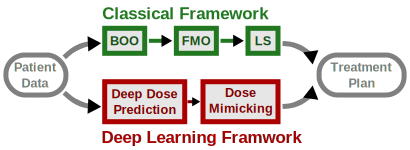
\includegraphics[width=\linewidth]{frameworks.pdf}
	\textit{
		\textbf{BOO:} Beam Orientation Optimization\\
		\textbf{FMO:} Fluence maps Optimization\\
		\textbf{LS:} Leaf Sequencing
	}
	\caption{Comparison of classical versus deep dose frameworks for the creation of treatment plans.}
	\label{fig:frameworks_comparison}
\end{figure}

\section{Long-Term Impact on Radiotherapy}
\paragraph{Treatments Standardization}
The widespread adoption of automated dosimetry will benefit patients and clinicians in the long term.
By standardizing treatment planning across centers, these systems will ensure that all patients, regardless of location, have access to high-quality treatments based on the best clinical practices.
This standardization is particularly important for isolated clinics or those with limited specialist availability, where clinicians may lack experience dealing with rare or complex cases.
Ultimately, this standardization will lead to more equitable access to advanced radiotherapy treatments, improving patient outcomes on a global scale.

\paragraph{Conclusion}
The research presented in this thesis has demonstrated the importance and feasibility of automating the dosimetry process in radiotherapy.
While there are challenges in clinical adoption and model scalability, the future of radiotherapy will undoubtedly move toward more automated systems.
Among the various frameworks explored, the deep dose approach provides the most promising pathway for effective automation, offering a blend of full automation and manual adjustment flexibility.
This balance will likely encourage gradual adoption, leading to a new era in radiotherapy where treatment planning is faster, more precise, and universally accessible.
